\documentclass[11pt]{beamer}

\usepackage[utf8]{inputenc}
\usepackage{tikz}

\begin{document}

\begin{frame}

\begin{center}

\vspace{-1cm}

\includegraphics[width=0.5\textwidth]{adjoint.png}

\textbf{\Large Industrial Placement Presentation}

\vspace{1cm}

David Kurniadi Angdinata

{\footnotesize MEng Mathematics and Computer Science 4}

{\scriptsize Friday, 04 October 2019}

\end{center}

\end{frame}

\begin{frame}{Company profile}

\pause

\begin{center}

\includegraphics[width=\textwidth]{citypoint.jpg}
\pause
\includegraphics[width=0.494\textwidth]{2016.jpg}
\pause
\includegraphics[width=0.494\textwidth]{2019.jpg}

\end{center}

\end{frame}

\begin{frame}{Company profile}

\pause

\begin{center}

\includegraphics[width=0.75\textwidth]{treasury.png}
\pause
\includegraphics[width=0.75\textwidth]{uplink.png}

\end{center}

\end{frame}

\begin{frame}{Organisation roles}

\pause

\begin{center}

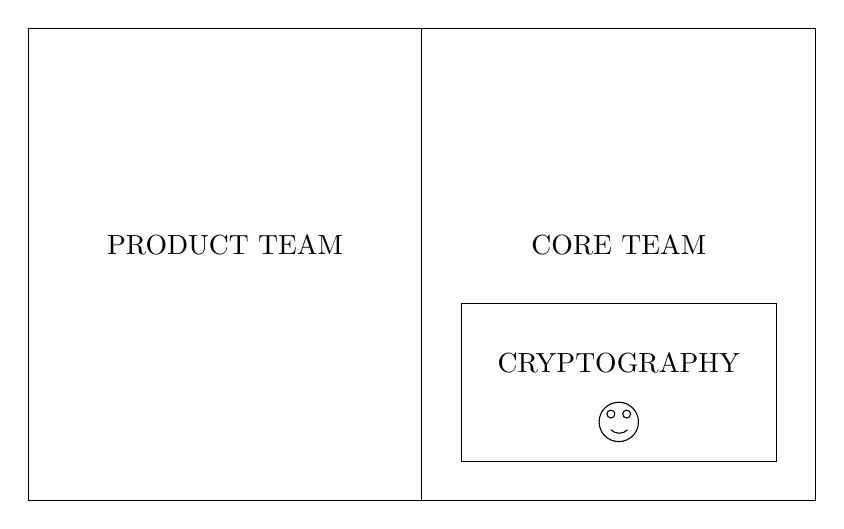
\begin{tikzpicture}
\draw (0, 0) rectangle node[above]{PRODUCT TEAM} (5, 6);
\pause
\draw (5, 0) rectangle node[above]{CORE TEAM} (10, 6);
\pause
\draw (5.5, 0.5) rectangle node[above]{CRYPTOGRAPHY} (9.5, 2.5);
\draw (7.5, 1) circle (0.25);
\draw (7.4, 1.1) circle (0.05);
\draw (7.6, 1.1) circle (0.05);
\draw (7.4, 0.9) arc (-135:-45:0.15);
\end{tikzpicture}

\end{center}

\end{frame}

\begin{frame}{Organisation roles}

\pause

\begin{center}

\includegraphics[width=\textwidth]{github.png}

\end{center}

\end{frame}

\begin{frame}{Cryptography roadmap}

\pause

\begin{center}

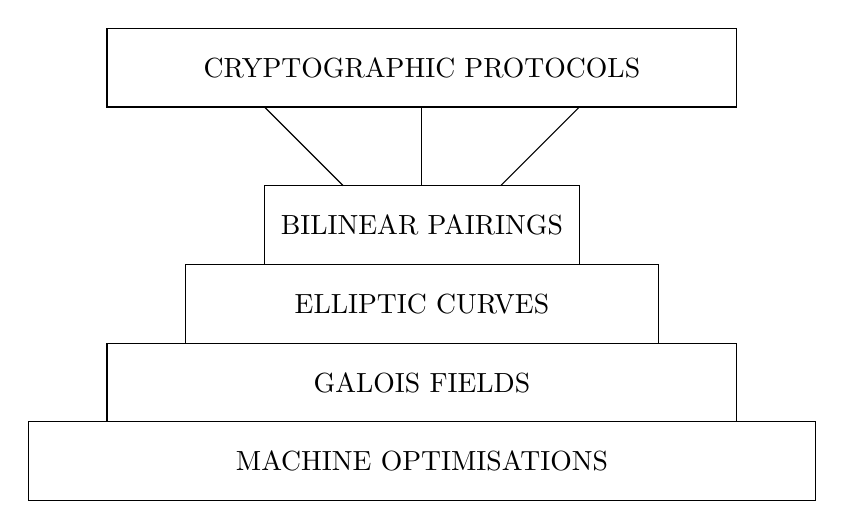
\begin{tikzpicture}
\draw (0, 0) rectangle node{MACHINE OPTIMISATIONS} (10, 1);
\pause
\draw (1, 1) rectangle node{GALOIS FIELDS} (9, 2);
\pause
\draw (2, 2) rectangle node{ELLIPTIC CURVES} (8, 3);
\pause
\draw (3, 3) rectangle node{BILINEAR PAIRINGS} (7, 4);
\pause
\draw (4, 4) -- (3, 5);
\draw (5, 4) -- (5, 5);
\draw (6, 4) -- (7, 5);
\draw (1, 5) rectangle node{CRYPTOGRAPHIC PROTOCOLS} (9, 6);
\end{tikzpicture}

\end{center}

\end{frame}

\begin{frame}{Cryptography roadmap}

\pause

\begin{center}

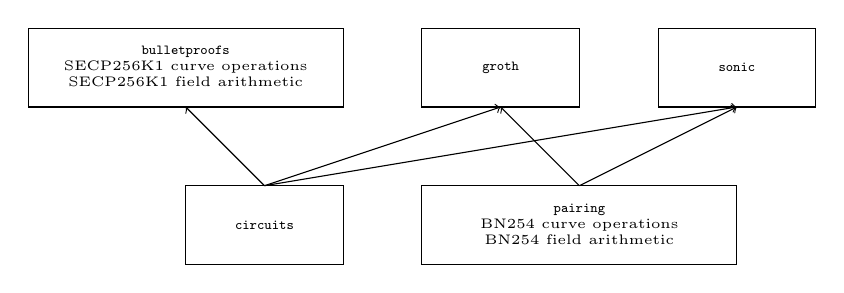
\begin{tikzpicture}
\draw (-3, 0) rectangle node{\tiny \texttt{circuits}} (-1, 1);
\draw (0, 0) rectangle node[above]{\tiny \texttt{pairing}} node{\tiny BN254 curve operations} node[below]{\tiny BN254 field arithmetic} (4, 1);
\pause
\draw [->] (-2, 1) -- (-3, 2);
\draw [->] (-2, 1) -- (4, 2);
\draw [->] (2, 1) -- (4, 2);
\draw (-5, 2) rectangle node[above]{\tiny \texttt{bulletproofs}} node{\tiny SECP256K1 curve operations} node[below]{\tiny SECP256K1 field arithmetic} (-1, 3);
\draw (3, 2) rectangle node{\tiny \texttt{sonic}} (5, 3);
\pause
\draw [->] (-2, 1) -- (1, 2);
\draw [->] (2, 1) -- (1, 2);
\draw (0, 2) rectangle node{\tiny \texttt{groth}} (2, 3);
\end{tikzpicture}

\end{center}

\end{frame}

\begin{frame}{An efficient library of Galois fields}

\pause

\begin{center}

\includegraphics[width=\textwidth]{galois-field.png}

\end{center}

\pause

\begin{itemize}[<+->]
\item Prime fields and extension fields
\item Extensive usage of type system
\item Slow performance of binary fields
\item Square roots and scalar multiplication
\item Heavy compile-time and run-time optimisations
\end{itemize}

\end{frame}

\begin{frame}{An efficient library of Galois fields}

\begin{center}

\only<1>{
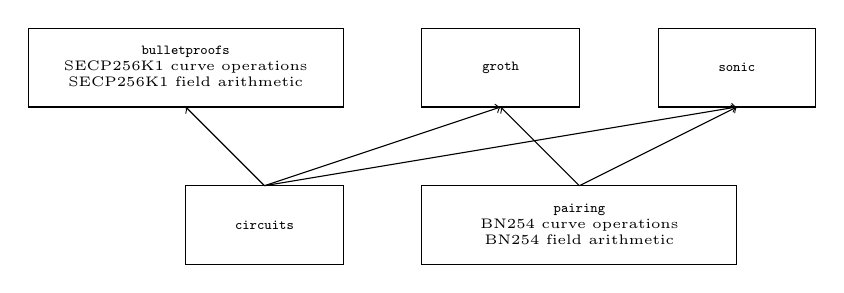
\begin{tikzpicture}
\draw (-3, 0) rectangle node{\tiny \texttt{circuits}} (-1, 1);
\draw (0, 0) rectangle node[above]{\tiny \texttt{pairing}} node{\tiny BN254 curve operations} node[below]{\tiny BN254 field arithmetic} (4, 1);
\draw [->] (-2, 1) -- (-3, 2);
\draw [->] (-2, 1) -- (1, 2);
\draw [->] (-2, 1) -- (4, 2);
\draw [->] (2, 1) -- (1, 2);
\draw [->] (2, 1) -- (4, 2);
\draw (-5, 2) rectangle node[above]{\tiny \texttt{bulletproofs}} node{\tiny SECP256K1 curve operations} node[below]{\tiny SECP256K1 field arithmetic} (-1, 3);
\draw (0, 2) rectangle node{\tiny \texttt{groth}} (2, 3);
\draw (3, 2) rectangle node{\tiny \texttt{sonic}} (5, 3);
\end{tikzpicture}
}
\only<2-3>{
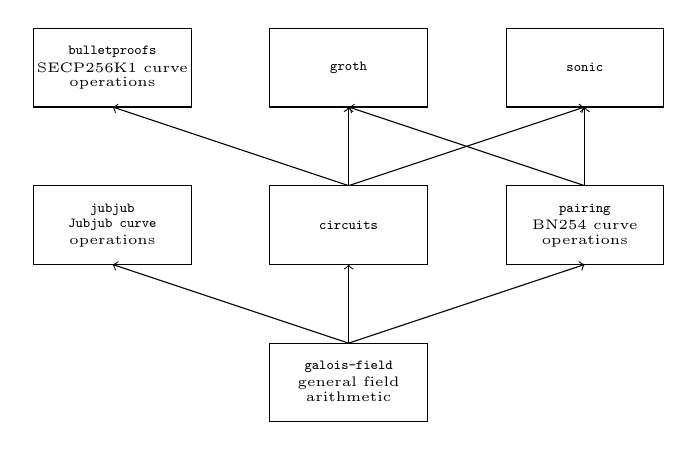
\begin{tikzpicture}
\draw (0, 0) rectangle node[above]{\tiny \texttt{galois-field}} node{\tiny general field} node[below]{\tiny arithmetic} (2, 1);
\draw [->] (1, 1) -- (1, 2);
\draw [->] (1, 1) -- (4, 2);
\draw (0, 2) rectangle node{\tiny \texttt{circuits}} (2, 3);
\draw [->] (1, 3) -- (-2, 4);
\draw [->] (1, 3) -- (1, 4);
\draw [->] (1, 3) -- (4, 4);
\draw (3, 2) rectangle node[above]{\tiny \texttt{pairing}} node{\tiny BN254 curve} node[below]{\tiny operations} (5, 3);
\draw [->] (4, 3) -- (1, 4);
\draw [->] (4, 3) -- (4, 4);
\draw (-3, 4) rectangle node[above]{\tiny \texttt{bulletproofs}} node{\tiny SECP256K1 curve} node[below]{\tiny operations} (-1, 5);
\draw (0, 4) rectangle node{\tiny \texttt{groth}} (2, 5);
\draw (3, 4) rectangle node{\tiny \texttt{sonic}} (5, 5);
\only<3>{
\draw [->] (1, 1) -- (-2, 2);
\draw (-3, 2) rectangle node[above]{\tiny \texttt{jubjub}} node{\tiny \texttt{Jubjub curve}} node[below]{\tiny operations} (-1, 3);
}
\end{tikzpicture}
}

\end{center}

\end{frame}

\begin{frame}{A universal library of elliptic curves}

\pause

\begin{center}

\includegraphics[width=\textwidth]{elliptic-curve.png}

\end{center}

\pause

\begin{itemize}[<+->]
\item Eighty elliptic curve domain parameters
\item Elliptic curve multi-parameter type class
\item Elliptic curve point associated type
\item Elliptic curve point addition formulas
\item Elliptic curve source code generator
\end{itemize}

\end{frame}

\begin{frame}{A universal library of elliptic curves}

\begin{center}

\only<1>{
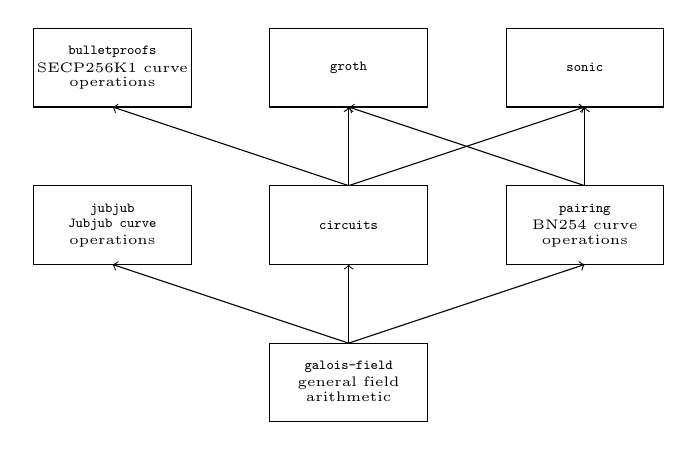
\begin{tikzpicture}
\draw (0, 0) rectangle node[above]{\tiny \texttt{galois-field}} node{\tiny general field} node[below]{\tiny arithmetic} (2, 1);
\draw [->] (1, 1) -- (-2, 2);
\draw [->] (1, 1) -- (1, 2);
\draw [->] (1, 1) -- (4, 2);
\draw (-3, 2) rectangle node[above]{\tiny \texttt{jubjub}} node{\tiny \texttt{Jubjub curve}} node[below]{\tiny operations} (-1, 3);
\draw (0, 2) rectangle node{\tiny \texttt{circuits}} (2, 3);
\draw [->] (1, 3) -- (-2, 4);
\draw [->] (1, 3) -- (1, 4);
\draw [->] (1, 3) -- (4, 4);
\draw (3, 2) rectangle node[above]{\tiny \texttt{pairing}} node{\tiny BN254 curve} node[below]{\tiny operations} (5, 3);
\draw [->] (4, 3) -- (1, 4);
\draw [->] (4, 3) -- (4, 4);
\draw (-3, 4) rectangle node[above]{\tiny \texttt{bulletproofs}} node{\tiny SECP256K1 curve} node[below]{\tiny operations} (-1, 5);
\draw (0, 4) rectangle node{\tiny \texttt{groth}} (2, 5);
\draw (3, 4) rectangle node{\tiny \texttt{sonic}} (5, 5);
\end{tikzpicture}
}
\only<2-3>{
\begin{tikzpicture}
\draw (0, 0) rectangle node[above]{\tiny \texttt{galois-field}} node{\tiny general field} node[below]{\tiny arithmetic} (2, 1);
\draw [->] (1, 1) -- (-1, 3);
\draw [->] (1, 1) -- (2, 2);
\draw (-2, 3) rectangle node{\tiny \texttt{circuits}} (0, 4);
\draw [->] (-1, 4) -- (-2, 6);
\draw [->] (-1, 4) -- (1, 6);
\draw [->] (-1, 4) -- (4, 6);
\draw (1, 2) rectangle node[above]{\tiny \texttt{elliptic-curve}} node{\tiny general curve} node[below]{\tiny operations} (3, 3);
\draw [->] (2, 3) -- (-2, 6);
\draw [->] (2, 3) -- (3, 4);
\draw (2, 4) rectangle node{\tiny \texttt{pairing}} (4, 5);
\draw [->] (3, 5) -- (1, 6);
\draw [->] (3, 5) -- (4, 6);
\draw (-3, 6) rectangle node{\tiny \texttt{bulletproofs}} (-1, 7);
\only<2>{
\draw (0, 6) rectangle node{\tiny \texttt{groth}} (2, 7);
\draw (3, 6) rectangle node{\tiny \texttt{sonic}} (5, 7);
}
\only<3>{
\draw (0, 6) rectangle node[above]{\tiny \texttt{groth}} node{\tiny BN254 pairing} node[below]{\tiny algorithms} (2, 7);
\draw (3, 6) rectangle node[above]{\tiny \texttt{sonic}} node{\tiny BLS12-381 pairing} node[below]{\tiny algorithms} (5, 7);
}
\end{tikzpicture}
}

\end{center}

\end{frame}

\begin{frame}{A polymorphic library of bilinear pairings}

\pause

\begin{center}

\includegraphics[width=\textwidth]{pairing.png}

\end{center}

\pause

\begin{itemize}[<+->]
\item Pairing for BN and BLS
\item General bilinear pairing type class
\item General optimal ate pairing algorithm
\item Seven elliptic curve bilinear pairings
\item BN elliptic curve hashing function
\end{itemize}

\end{frame}

\begin{frame}{A polymorphic library of bilinear pairings}

\begin{center}

\only<1>{
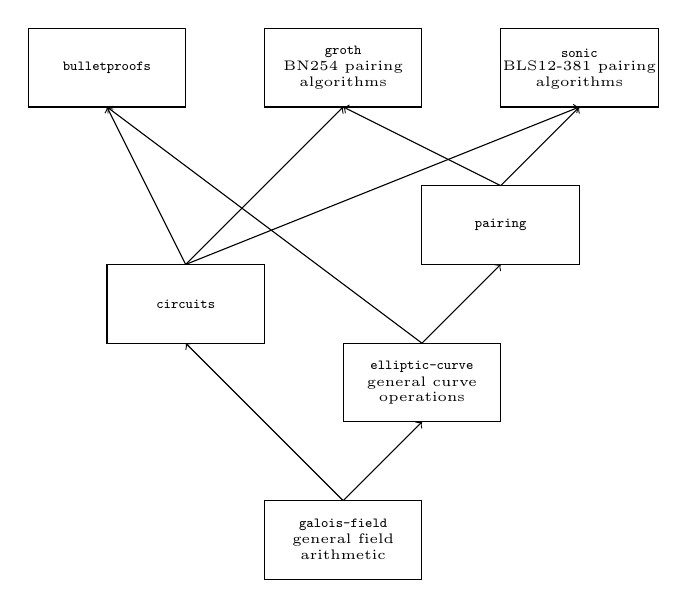
\begin{tikzpicture}
\draw (0, 0) rectangle node[above]{\tiny \texttt{galois-field}} node{\tiny general field} node[below]{\tiny arithmetic} (2, 1);
\draw [->] (1, 1) -- (-1, 3);
\draw [->] (1, 1) -- (2, 2);
\draw (-2, 3) rectangle node{\tiny \texttt{circuits}} (0, 4);
\draw [->] (-1, 4) -- (-2, 6);
\draw [->] (-1, 4) -- (1, 6);
\draw [->] (-1, 4) -- (4, 6);
\draw (1, 2) rectangle node[above]{\tiny \texttt{elliptic-curve}} node{\tiny general curve} node[below]{\tiny operations} (3, 3);
\draw [->] (2, 3) -- (-2, 6);
\draw [->] (2, 3) -- (3, 4);
\draw (2, 4) rectangle node{\tiny \texttt{pairing}} (4, 5);
\draw [->] (3, 5) -- (1, 6);
\draw [->] (3, 5) -- (4, 6);
\draw (-3, 6) rectangle node{\tiny \texttt{bulletproofs}} (-1, 7);
\draw (0, 6) rectangle node[above]{\tiny \texttt{groth}} node{\tiny BN254 pairing} node[below]{\tiny algorithms} (2, 7);
\draw (3, 6) rectangle node[above]{\tiny \texttt{sonic}} node{\tiny BLS12-381 pairing} node[below]{\tiny algorithms} (5, 7);
\end{tikzpicture}
}
\only<2>{
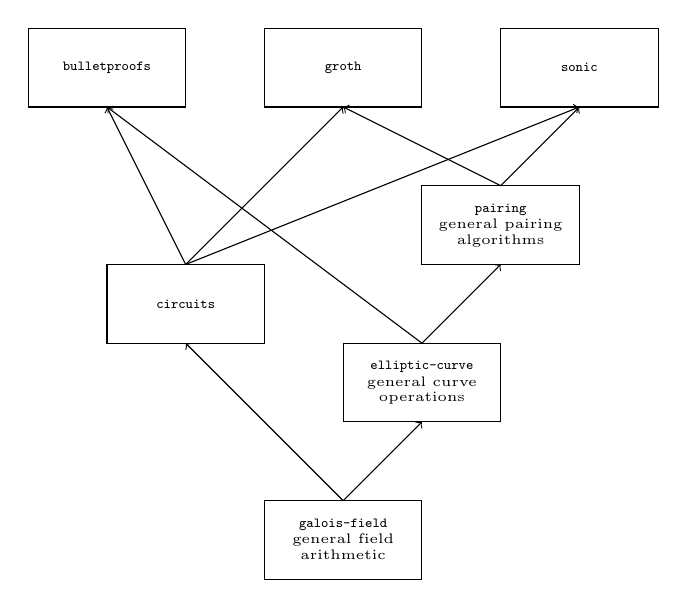
\begin{tikzpicture}
\draw (0, 0) rectangle node[above]{\tiny \texttt{galois-field}} node{\tiny general field} node[below]{\tiny arithmetic} (2, 1);
\draw [->] (1, 1) -- (-1, 3);
\draw [->] (1, 1) -- (2, 2);
\draw (-2, 3) rectangle node{\tiny \texttt{circuits}} (0, 4);
\draw [->] (-1, 4) -- (-2, 6);
\draw [->] (-1, 4) -- (1, 6);
\draw [->] (-1, 4) -- (4, 6);
\draw (1, 2) rectangle node[above]{\tiny \texttt{elliptic-curve}} node{\tiny general curve} node[below]{\tiny operations} (3, 3);
\draw [->] (2, 3) -- (-2, 6);
\draw [->] (2, 3) -- (3, 4);
\draw (2, 4) rectangle node[above]{\tiny \texttt{pairing}} node{\tiny general pairing} node[below]{\tiny algorithms} (4, 5);
\draw [->] (3, 5) -- (1, 6);
\draw [->] (3, 5) -- (4, 6);
\draw (-3, 6) rectangle node{\tiny \texttt{bulletproofs}} (-1, 7);
\draw (0, 6) rectangle node{\tiny \texttt{groth}} (2, 7);
\draw (3, 6) rectangle node{\tiny \texttt{sonic}} (5, 7);
\end{tikzpicture}
}

\end{center}

\end{frame}

\begin{frame}{Conclusion}

\pause

Powerful type system in Haskell

\pause

\vspace{1cm}

Crucial performance optimisations in Haskell

\pause

\vspace{1cm}

Mathematical background behind zero-knowledge proofs

\pause

\vspace{1cm}

Cryptographic applications of number theory

\pause

\vspace{1cm}

Collaborative communication and productivity management

\end{frame}

\begin{frame}

\begin{center}

\includegraphics[width=0.5\textwidth]{adjoint.png}

\textbf{\Huge THANK YOU}

\end{center}
    
\end{frame}

\end{document}